\subsection{数据检查与运行环境}
课程数据包包含 bottle（瓶子）、cable（电缆）、leather（皮革）、pill（药片）、tile（瓷砖）和 transistor（晶体管）六类，每类 100 张，共 600 张 RGB 图像。原始分辨率为 $1024\times1024$ 的图像有 300 张，$800\times800$、$900\times900$ 和 $840\times840$ 各有 100 张。所有文件均成功解码，文件名一一对应官方标签。600 个文件的 SHA-256 各不相同，按 RGB 解码像素及尺寸计算的哈希也未发现完全重复图像；这一检查不排除近重复或同一场景中的相似样本。

实验于 2026 年 11 月 26 日在 Windows 11 上完成，使用 Python 3.12.14、PyTorch 2.15.0+cpu、Torchvision 0.29.2+cpu、NumPy 2.5.5、SciPy 1.18.1、scikit-learn 1.9.1、scikit-image 0.26.0 和 Pillow 13.0.0。编码采用 CPU、四个计算线程，批次大小为 16。神经网络前向计算启用确定性算法，逐行归一化和聚类输入使用 float64。使用官方 \texttt{resnet18-f37072fd.pth} 权重文件，并核对其完整 SHA-256，保证本地权重与指定预训练版本一致。

程序依次保存配置、特征、聚类结果、中心和内部指标，记录这些产物的哈希后，再读取类别标签进行外部评价。配置文件固定主方法 B 和种子 11。保存的日志时间和封存清单提供执行轨迹，但仅凭哈希不能独立证明历史执行的先后顺序；它们主要支持后续核对产物是否发生变化。

\subsection{定量结果与稳定性}
\label{sec:task1-quantitative}
全部 16 次运行均得到六个大小为 100 的簇，ACC、ARI 和 NMI 均为 1。表~\ref{tab:task1-internal} 汇总结果。三种 K-means 方案各运行五个种子，三个外部指标的样本标准差均为 0；每种方案内部十对划分的 ARI 也全部为 1。Ward 只进行确定性单次运行，不报告随机重复的标准差或种子稳定性。

主方法种子 11 的最优编号匹配为：簇 0 对应瓶子、簇 1 对应瓷砖、簇 2 对应药片、簇 3 对应皮革、簇 4 对应晶体管、簇 5 对应电缆。重排后的混淆矩阵如图~\ref{fig:task1-confusion} 所示，各类 100 张全部位于对角线。这里的 100\% 表示这批图像的划分与提供标签一致，不是独立测试集上的分类准确率。

\begin{figure}[t]
\centering
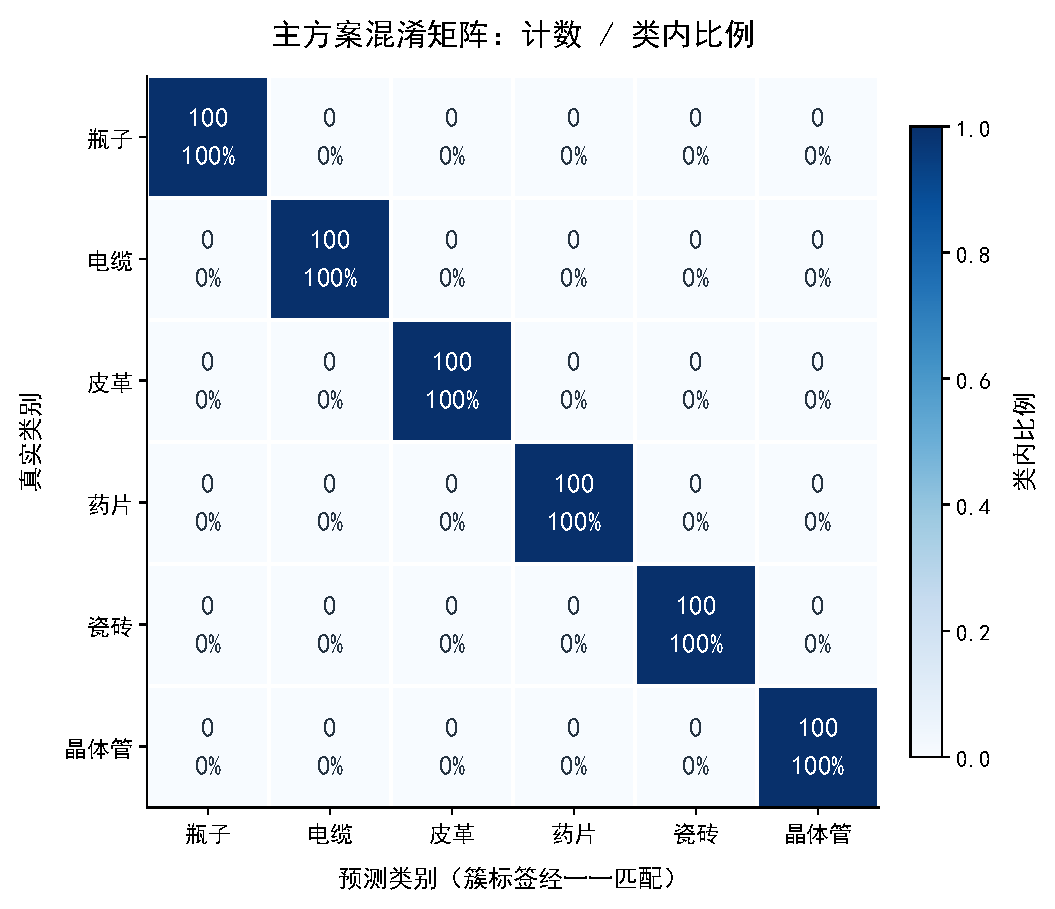
\includegraphics[width=\linewidth]{figures/confusion-matrix.pdf}
\Description{主方案经一对一编号匹配后的六类混淆矩阵，对角线均为 100，其他位置均为 0。}
\caption{主方法种子 11 的匹配后混淆矩阵。颜色为类内比例，单元格同时标注样本数和比例。}
\label{fig:task1-confusion}
\end{figure}

传统颜色纹理基线同样达到满分，是解释本次结果的关键。它说明在本数据和既定表示下，类别结构已经容易分开；实验没有证明冻结深度特征比传统特征具有更高的聚类质量，也没有证据支持通过继续增加模型复杂度改善这组外部指标。主方法仍保持预先指定的 B，不因结果同分而事后改变方法叙述。

\subsection{对照分析与计算开销}
表~\ref{tab:task1-internal} 给出内部指标和聚类计时。B 与 D 在相同特征上得到相同划分，所以轮廓系数、CH 和 DB 在显示精度下也相同。A 的轮廓系数为 0.8374，B 为 0.6783，但两者使用不同表示，这一数值差异不能解释为 A 的语义识别能力更强；外部评价实际没有差异。

\begin{table*}[t]
\caption{全部预定方案的评价与聚类时间。A、B、C 为五个固定种子的均值，外部指标标准差均为零；D 为单次运行。时间为均值 $\pm$ 样本标准差，仅含聚类器构造与拟合预测，不含图像编码、PCA 拟合、指标计算和绘图。}
\label{tab:task1-internal}
\centering
\setlength{\tabcolsep}{4.5pt}
\begin{tabular}{lcccccc}
\toprule
方案 & 维度 & ACC / ARI / NMI & 轮廓系数 $\uparrow$ & CH $\uparrow$ & DB $\downarrow$ & 聚类时间（秒）\\
\midrule
A：颜色纹理 + K-means & 138 & $1/1/1$ & 0.8374 & 2803.44 & 0.3333 & $0.0670\pm0.0193$\\
B：深度特征 + K-means & 512 & $1/1/1$ & 0.6783 & 961.20 & 0.5398 & $0.1050\pm0.0154$\\
C：深度特征 + PCA + K-means & 64 & $1/1/1$ & 0.7203 & 1222.98 & 0.4692 & $0.0455\pm0.0014$\\
D：深度特征 + Ward & 512 & $1/1/1$ & 0.6783 & 961.20 & 0.5398 & 0.4540\\
\bottomrule
\end{tabular}
\end{table*}

PCA 的 64 个主成分保留了 97.3351\% 的样本方差，特征维度由 512 降为 64，减少 87.5\%。C 的外部指标与 B 相同，因此这里观察到的是在保持本批次划分的同时压缩表示，而不是准确率提升。PCA 后重新归一化改变了距离几何，其内部指标变化不能单独证明语义信息增加。

对 $N$ 个 $d$ 维样本、$K$ 个中心，Lloyd 方法每轮计算样本到中心距离的主要代价随 $NKd$ 增长。其他条件相同时，64 维表示的这一部分坐标运算量为 512 维的八分之一。保存为 float64 稠密数组时，$600\times512$ 个特征约占 2.34 MiB，$600\times64$ 约占 0.293 MiB；这里不包含模型参数、图像和其他中间量。

本次 C 的聚类平均时间为 0.0455 秒，B 为 0.1050 秒；Ward 单次为 0.4540 秒。由于规模较小、计时易受系统状态影响，而且未单独计时 PCA 拟合，这些数值只用于描述本次运行，不能当作完整流程的普遍加速结论。图像读取、数据校验、两类特征提取及相关准备合计用时 54.59 秒，未分别计量传统分支与 ResNet 分支，不能把该数值称作纯 ResNet 推理时间。

\subsection{可视化与结果解释}
图~\ref{fig:task1-embedding} 对主方案的 512 维归一化特征作无标签二维 PCA 投影。左右两图使用完全相同的坐标，分别按真实类别、匹配后的预测簇着色。前两个主成分解释 28.65\% 和 20.51\% 的方差，合计约 49.16\%。两图颜色分组一致与外部评价结果相符，但二维投影只保留部分变化，不能替代在原 512 维空间计算距离和聚类。

\begin{figure*}[t]
\centering
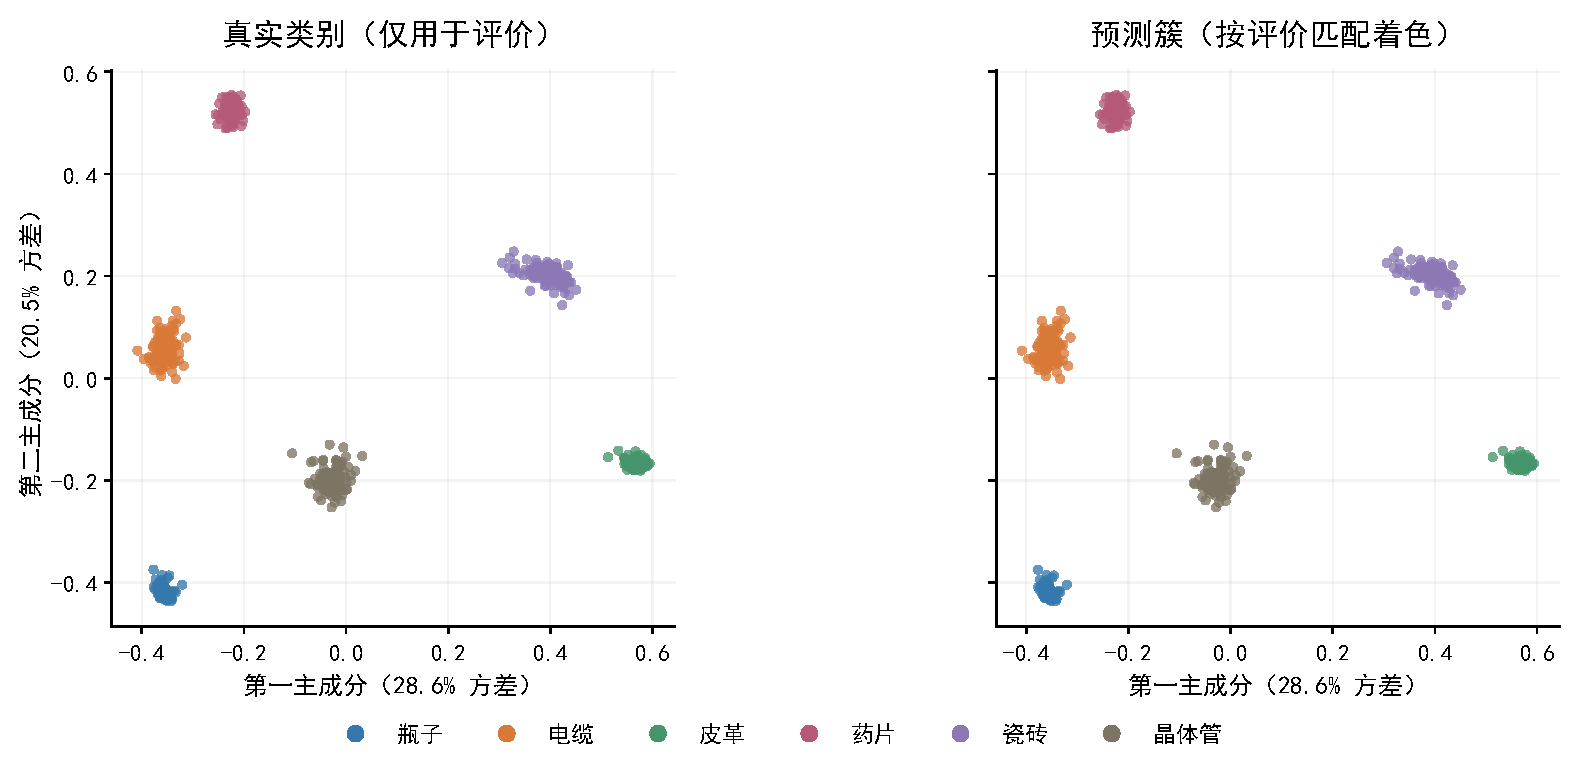
\includegraphics[width=0.95\textwidth]{figures/cluster-embedding.pdf}
\Description{归一化深度特征的同一二维 PCA 坐标分别按真实类别和匹配后的预测簇着色，两种着色一致；投影未使用类别标签拟合。}
\caption{主方案的二维 PCA 展示。编号匹配仅用于统一显示颜色，聚类仍在 512 维表示上完成。}
\label{fig:task1-embedding}
\end{figure*}

图~\ref{fig:task1-examples} 从每个预测簇选出距离该簇深度特征中心最近的两张图像，距离相同时按文件名排序。这种选法由特征与预测簇决定，再附上真实类别作为说明，没有按“识别正确”筛选展示图片。样例可见对象形态、主色调、背景及纹理的类别间差异，例如瓶子与药片的背景亮度、皮革与瓷砖的纹理形态不同。结合传统特征也达到满分，可以提出这些外观线索可能有帮助的解释；本实验没有做背景替换、前景分割或遮挡控制，因而不能断定背景是结果的原因。

\begin{figure*}[t]
\centering
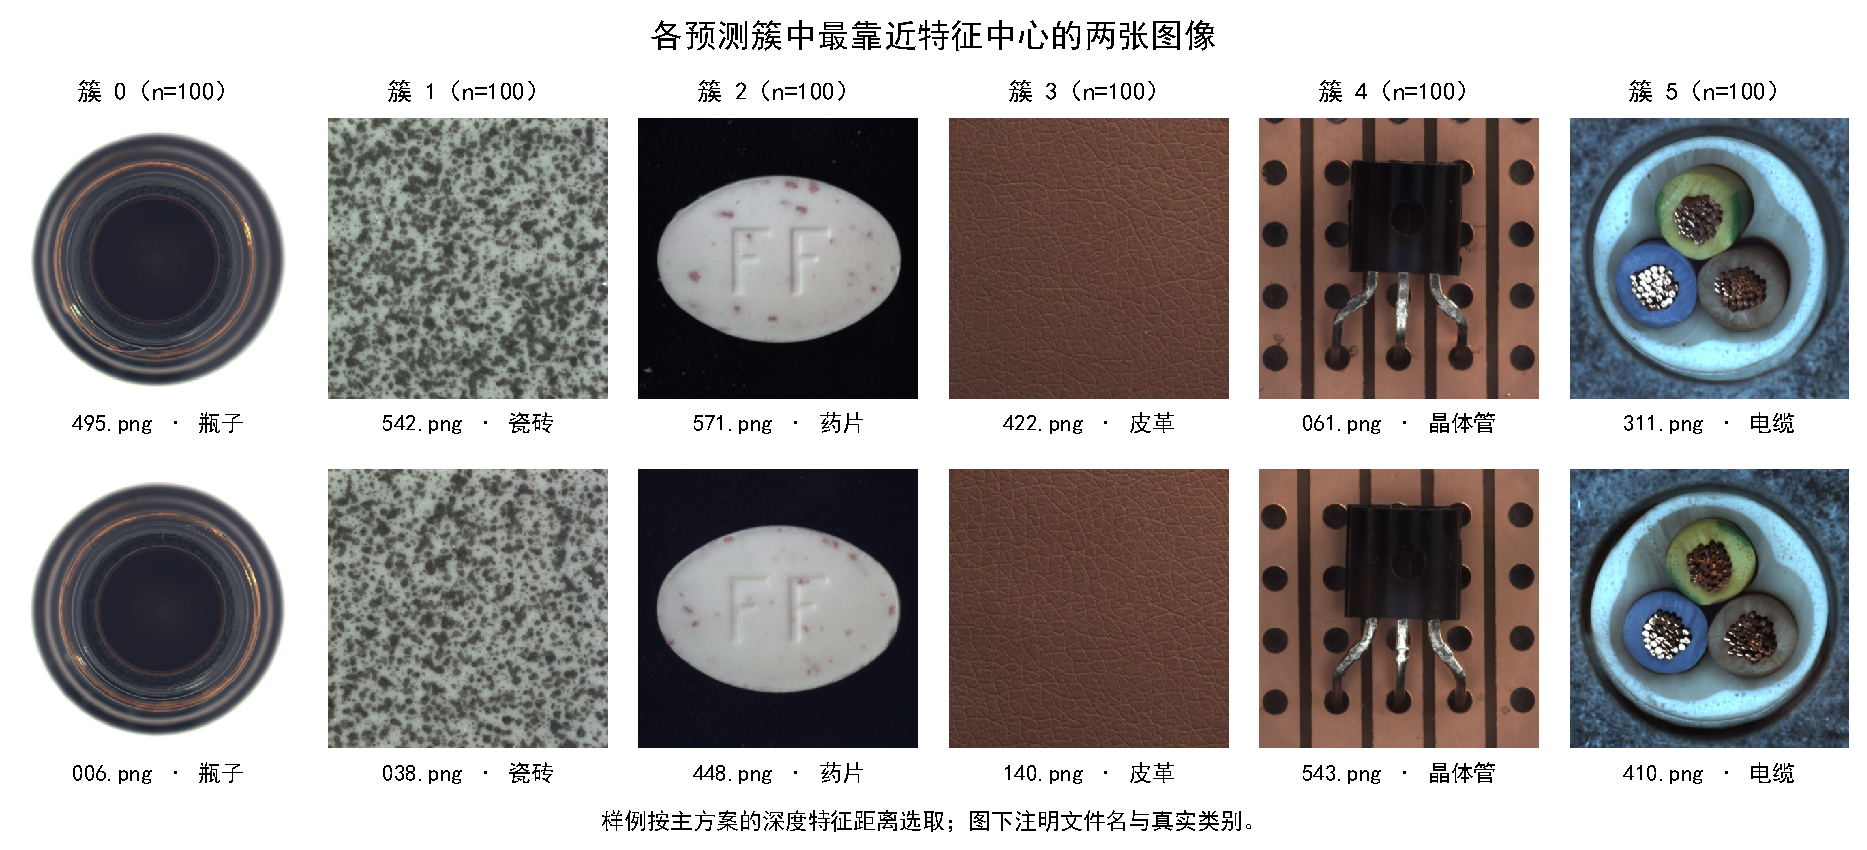
\includegraphics[width=0.98\textwidth]{figures/cluster-examples.pdf}
\Description{六个预测簇各展示距特征中心最近的两张图像，分别为瓶子、瓷砖、药片、皮革、晶体管和电缆，并标注文件名。}
\caption{主方案各簇的中心邻近样例。每簇含 100 张图像，展示的两张只用于解释外观，不能代表完整的数据扰动范围。}
\label{fig:task1-examples}
\end{figure*}

\FloatBarrier
\balance
\subsection{核验范围与局限}
独立核验脚本重新核对了封存产物的 SHA-256、600 个官方文件名、三组特征维度及单位范数、PCA 重建、16 组聚类输出和 15 组 K-means 的最近中心分配。程序按文件名重新读取官方标签，重建全部 16 组 ACC、ARI、算术平均熵归一化 NMI，并核对主方案逐图预测和混淆矩阵；\texttt{verification.json} 的状态为通过。该检查证明保存产物与评价计算相互一致；它不重新拟合聚类，也不独立证明日志记录的历史执行顺序。

\InputIfFileExists{sec/task1-feature-verification.tex}{}{}

本次结果有三项边界。第一，六类均衡且在现有表示下容易分开，不能由满分推断方法能处理外观近似类别、不均衡类别或异常噪声。第二，全部图像参与无标签拟合，没有新批次留出测试，五种子稳定也不等于对新图像或分布变化的稳定。第三，外部预训练可能提供与本题对象相关的知识，但没有从零训练或其他预训练来源的对照，不能分离这部分贡献。后续若需研究泛化，应增加独立批次、相似类别与背景控制实验，再使用预先固定的评价协议检验；这些实验未在本报告中实施。

\subsection{小结}
在课程提供的 600 张图像上，预定主方法及三个对照的全部 16 次运行均与六类标签划分一致，ACC、ARI、NMI 均为 1。传统基线同样达到满分，说明当前结果不足以证明深度方法具有性能优势。PCA 在不改变本批次外部结果的情况下将特征压缩为 64 维；Ward 与主方法同分。报告以固定方法、完整对照及可复核产物说明这一结果，将结论限定于已提供数据，不据此宣称新图像上的泛化能力。
